\begin{task}{2.2, Implementation of the neural network - Architecture Focus approach (20\%)}

\paragraph{Architectural focus}
The following results were completed before the first part of this task and we only later found out decreasing the batch size significantly together with removing unnecessary pedestrians and taking every frame allows us to recreate the results from the paper. This part of the task therefore mostly concerns itself with working in the context of mega-batches and an 80 frame sampling period.

\paragraph{Training procedure}
For the training we try the same procedure as the paper \cite{tordeux2020prediction}. For a given experiment taking different combinations of experiments. We take either all the data from an experiment type if it is only present in one split (B/C, C/B). In cases where it is present in multiple splits we do a 50/50 train test split and adjust the training set so it is roughly balanced. We always use the whole test set in a batch.

Afterwards we run k-fold bootstrapping (like cross-validation except we only use it to select the best model) on the train set to find the best parameters. We use all the datapoints in each batch because there are only tens of thousands of them.

The data in the paper is processed by taking one datapoint every 80 frames and getting the speed/ velocity by taking a point 16 frames in the future. We can better approximate the speed by taking the average of the speed in the eight previous and the eight next frames. We use one datapoint every 80 frames but decreasing the spacing does not impact model performance on the generalization experiments.

In  the paper they also talk about getting the Weidmann parameter's from the neural networks which is at odds with what the rest of their paper seems to say. We tried instead of directly predicting the speed, to predict the Weidmann model parameters and use Weidmann's equation to create predictions but this has abysmal results with any hyperparameters we could find. Another thing we tried was to predict 2 values and then take $x * exp(y)$. Both has higher or equal loss so in the experiments shown we only use the network with no activation at the end.

\paragraph{Trying to recreate the original results}
We were unable to recreate the original results even when using the original data processing in \ref{fig:original}. We only tried the NN3 architecture from the paper (it uses relative positions of the k nearest pedestrians and their mean spacing) as it has the best results. The paper did not mention whether the pedestrians that do not have enough neighbors should be removed so we assume they should not be (if they have at least two neighbors) and instead replace the values of these neighbors with zero and only calculate mean spacing from the neighbors they do have. When we later tried to remove the pedestrians without enough neighbors the model performance did not significantly change. For the number of neighbors we follow the example of the paper and use 10.

We use a weight decay of 0.2, learning rate of 1e-3, learning rate decay of 0.98 and run the training for 50 epochs. Later we also trying these architectures on our data \ref{fig:originalourdata}. We can see that the models produced using the method from the paper have comparable results.

\begin{figure}
    \centering
    \subfigure[(1,)]{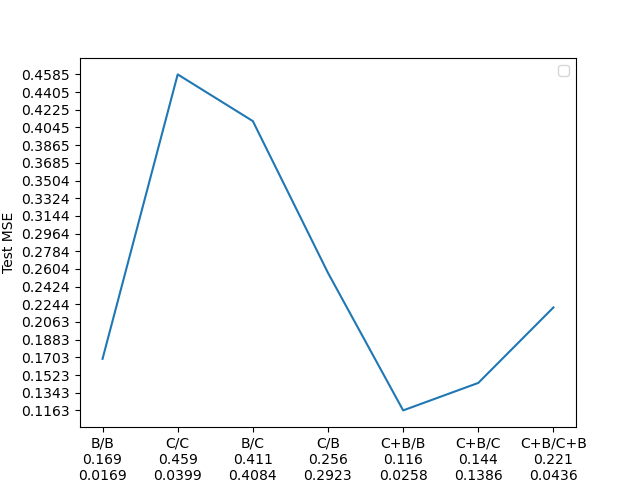
\includegraphics[width=0.3\textwidth]{images/original/1-0.001.png}}
    \subfigure[(2,)]{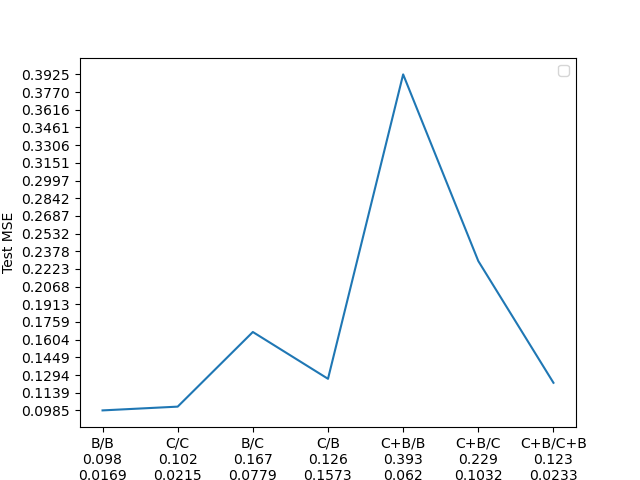
\includegraphics[width=0.3\textwidth]{images/original/2-0.001.png}}
    \subfigure[(3,)]{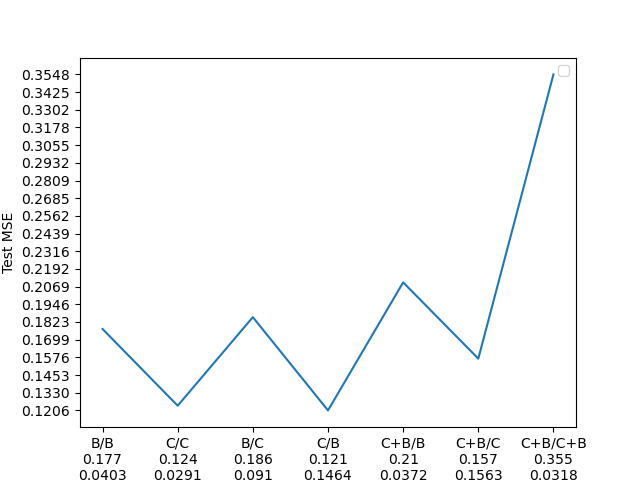
\includegraphics[width=0.3\textwidth]{images/original/3-0.001.png}}
    \subfigure[(5,2)]{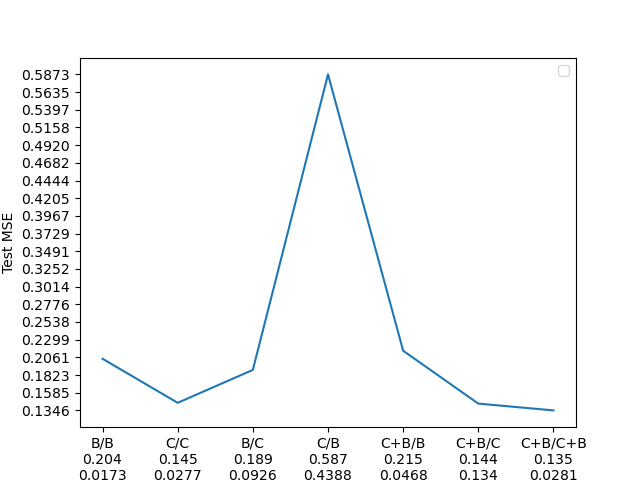
\includegraphics[width=0.3\textwidth]{images/original/5-2-0.001.png}}
    \subfigure[(5,3)]{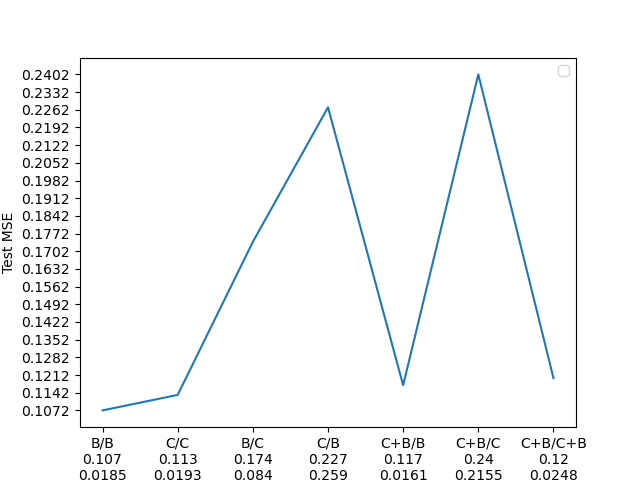
\includegraphics[width=0.3\textwidth]{images/original/5-3-0.001.png}}
    \subfigure[(6,3)]{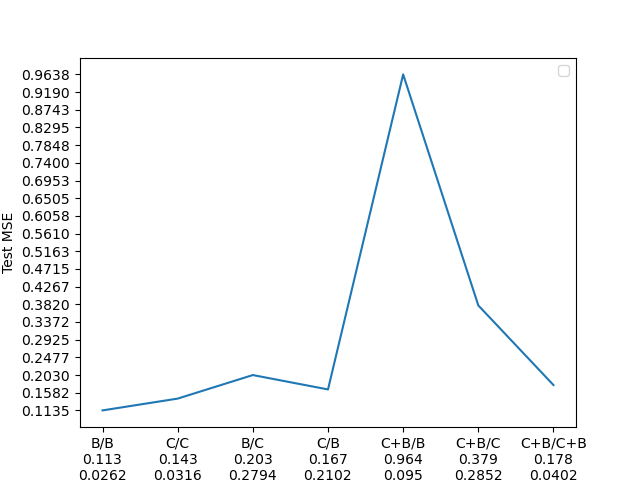
\includegraphics[width=0.3\textwidth]{images/original/6-3-0.001.png}}
    \subfigure[(10,4)]{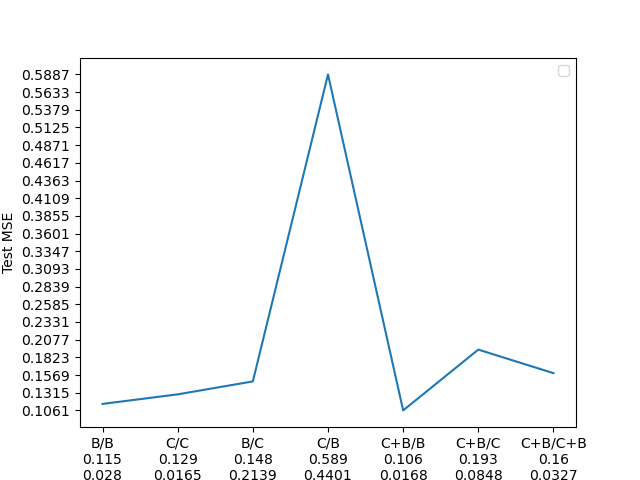
\includegraphics[width=0.3\textwidth]{images/original/10-4-0.001.png}}
    \caption{Every 80 frames looking 16 frames into the future using the NN3 architecture}
    \label{fig:original}
\end{figure}

\begin{figure}
    \centering
    \subfigure[(1,)]{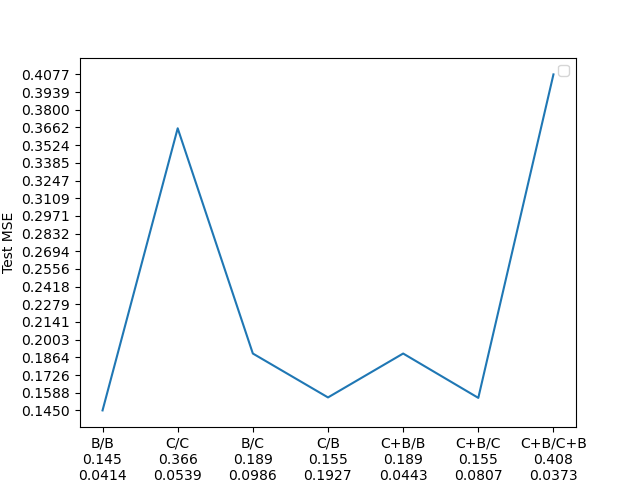
\includegraphics[width=0.3\textwidth]{images/originalourdata/1-0.001.png}}
    \subfigure[(2,)]{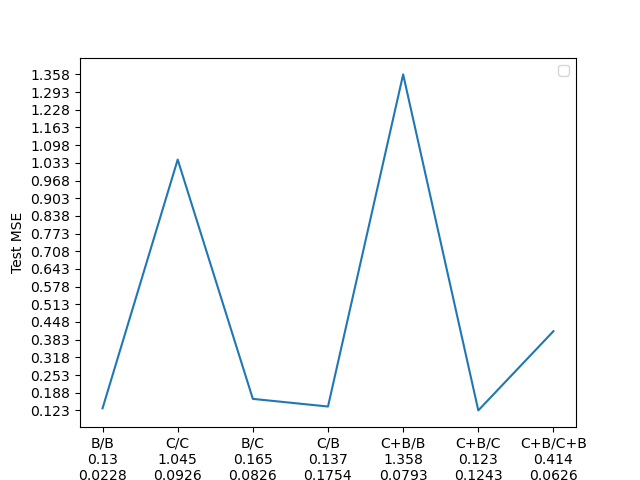
\includegraphics[width=0.3\textwidth]{images/originalourdata/2-0.001.png}}
    \subfigure[(3,)]{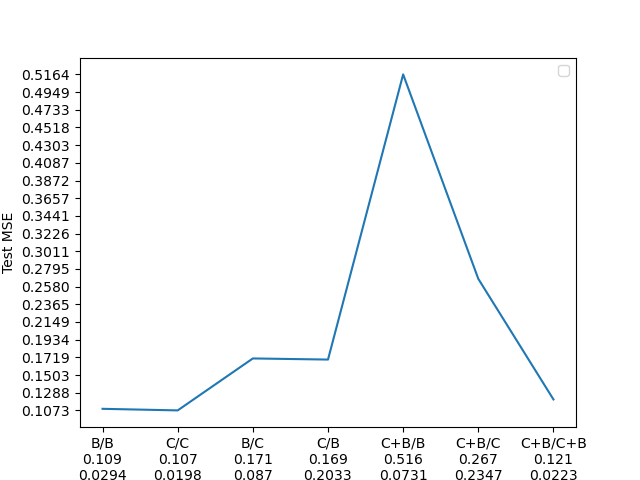
\includegraphics[width=0.3\textwidth]{images/originalourdata/3-0.001.png}}
    \subfigure[(5,2)]{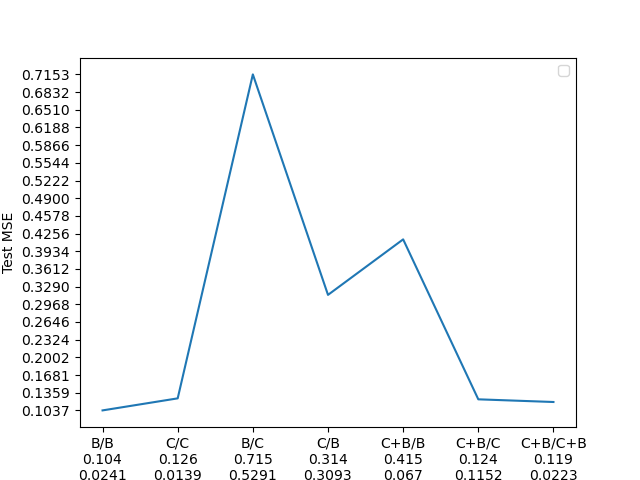
\includegraphics[width=0.3\textwidth]{images/originalourdata/5-2-0.001.png}}
    \subfigure[(5,3)]{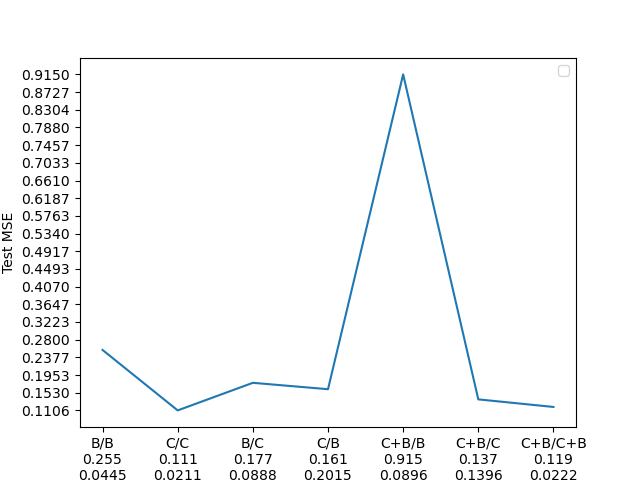
\includegraphics[width=0.3\textwidth]{images/originalourdata/5-3-0.001.png}}
    \subfigure[(6,3)]{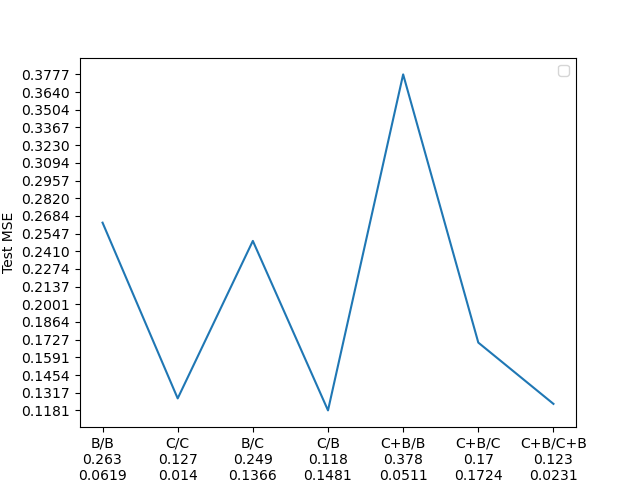
\includegraphics[width=0.3\textwidth]{images/originalourdata/6-3-0.001.png}}
    \subfigure[(10,4)]{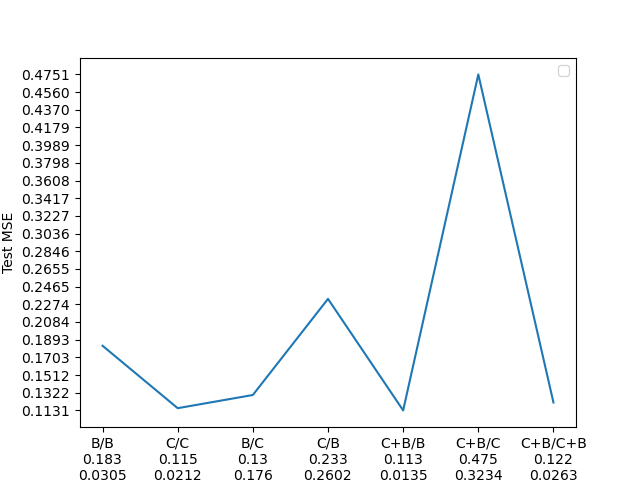
\includegraphics[width=0.3\textwidth]{images/originalourdata/10-4-0.001.png}}
    \caption{Every 80 frames taking average speed in 8 frame window behind and forward in time the NN3 architecture}
    \label{fig:originalourdata}
\end{figure}

\paragraph{Off the shelf second order optimization}
Since we are already using a massive fraction of the dataset each iteration the idea came up that we could simply use the whole dataset each iteration and use a second order method.

These are methods similar to the newton method and use the first and second derivatives. This is normally very unfortunate because it means we need $p^2$ space and $p^3$ time where $p$ is the usually very large number of parameters and of course we need to fit all the data and copies of the data for paramater purposes in the memory along with this.

The specific method we use is described in \cite{martens2020optimizing}. In the paper they say that while their method is derived in a different way than the newton method it can be seen as a generalization of it. The paper also talks about how important weight regularization can be for second order methods and seeing as our methods seem to fail to generalize that well these might be good to use. Because the convergence of these methods is quite slow we only attempt them on the NN4 and layer sizes [(3,), (4,2,), (5,2,), (5,3,), (6,3,), (10,4,)] and the C+B/C+B dataset.

 We use no weight decay, again a learning rate of 6e-2, learning rate decay of 0.98 and run the training for 50 epochs.
 
\begin{figure}
    \centering
    \subfigure[(3,)]{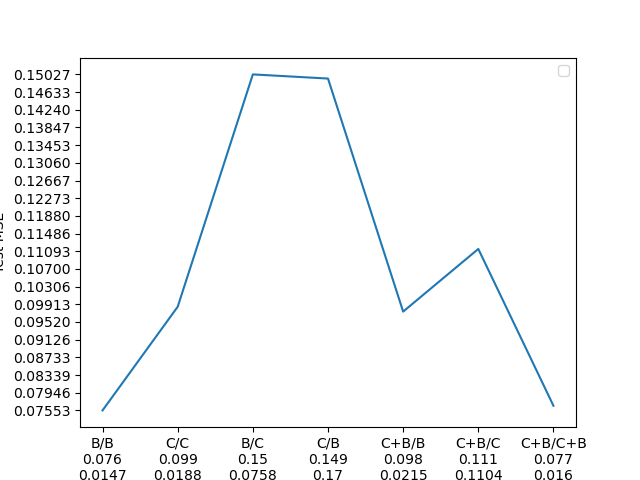
\includegraphics[width=0.3\textwidth]{images/secondorderoffshelf/3-0.06.png}}
    \subfigure[(5,2)]{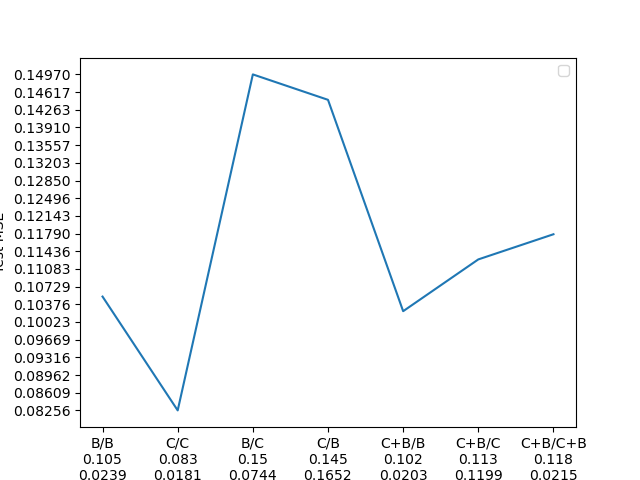
\includegraphics[width=0.3\textwidth]{images/secondorderoffshelf/5-2-0.06.png}}
    \subfigure[(5,3)]{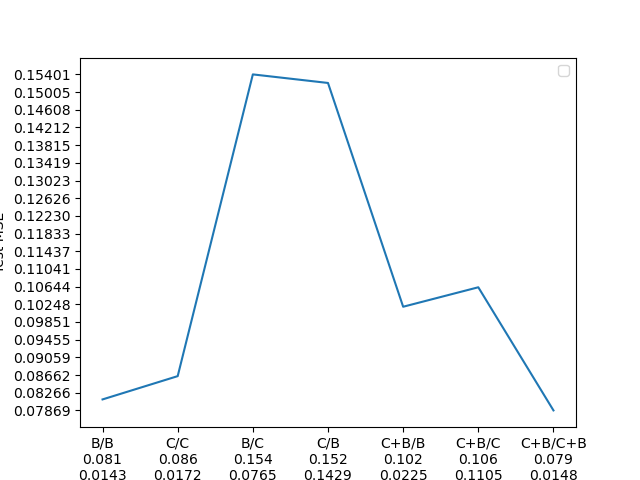
\includegraphics[width=0.3\textwidth]{images/secondorderoffshelf/5-3-0.06.png}}
    \subfigure[(6,3)]{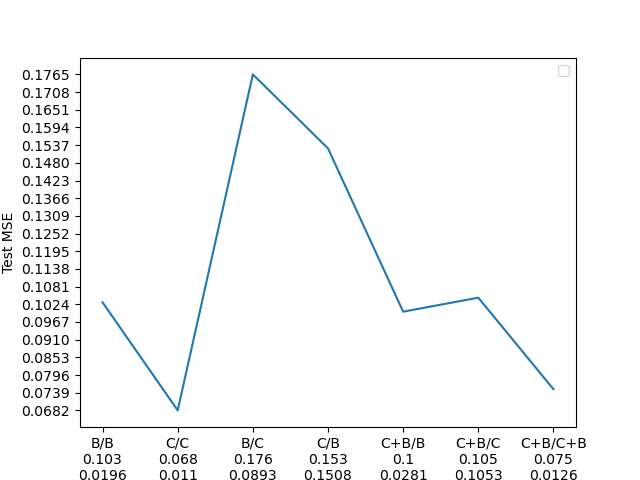
\includegraphics[width=0.3\textwidth]{images/secondorderoffshelf/6-3-0.06.png}}
    \subfigure[(10,4)]{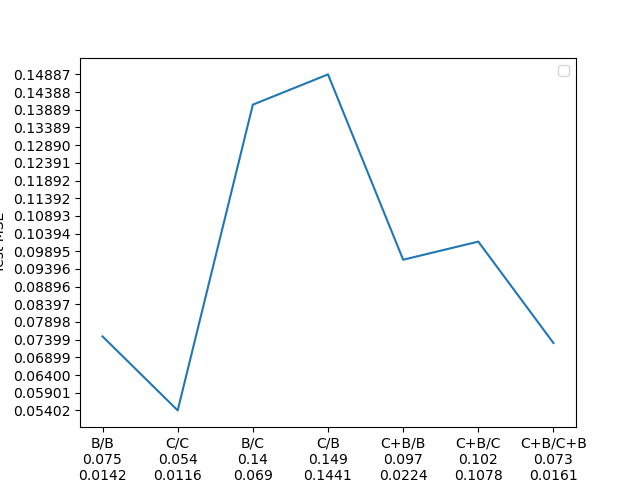
\includegraphics[width=0.3\textwidth]{images/secondorderoffshelf/10-4-0.06.png}}
    \caption{Every 80 frames taking average speed in 8 frame window behind and forward in time using the NN3 architecture and a second order optimizer with default arguements}
    \label{fig:secoroffshelf}
\end{figure}

As we can observe in Figure \ref{fig:secoroffshelf} our networks ouperform their architectures on this data with our parameters. Especially the large networks seem to scale better. This lead to the understandable desire to see how even larger networks would perform.

\paragraph{Second order parameter optimization and regularization}
We tried large networks, the MSE for the very simple C/C and B/B scenarios was even better but they generalized even worse.

To remedy this we try to use different optimizer parameters, most interesting is the regularization parameter and the momentum parameter. We also add our own L2 regularization directly to the loss as the method we use lacks it. We use all different parameters for each experiment and select the best network using the validation loss.

Eventually after increasing the number of parameters to (12,5,3) and the number of epochs up to 100 we get the following results. We use no weight decay, learning rate of 6e-2, learning rate decay of 0.98 and run the training. We are accumulating over up to 30 iterations (we still step in each iteration we just use all 30 last iterations).

\begin{figure}
\begin{center}
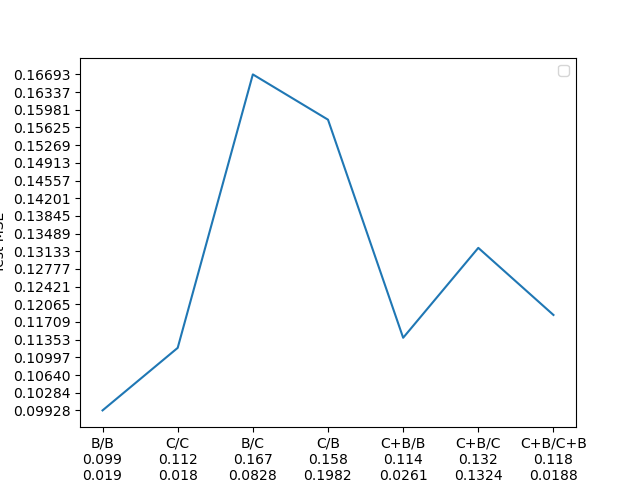
\includegraphics[width=0.3\textwidth]{images/12-5-3-0.05.png}
\end{center}
\caption{large network (12,5,3), second order optimization, regularization and less momentum}
\label{fig:regularization}
\end{figure}

As we see in Figure \ref{fig:regularization} there appears to be no significant change. This does not mean that there might not be a combination of parameters we did not try that wouldn't yield better results but because of time constraints we did not find it.

\paragraph{Variation method}
To try to further increase generalization we try to use a variational architecture. Instead of doing just fully connected layers we use $l*l+l$ neurons to create the variance matrix and the mean for the gaussian. This seems to have more potential to fit the data but generalizes even worse \ref{fig:variational}. One interesting thing is that while the resulting model has more parameters it also requires less training.

\begin{figure}
\begin{center}
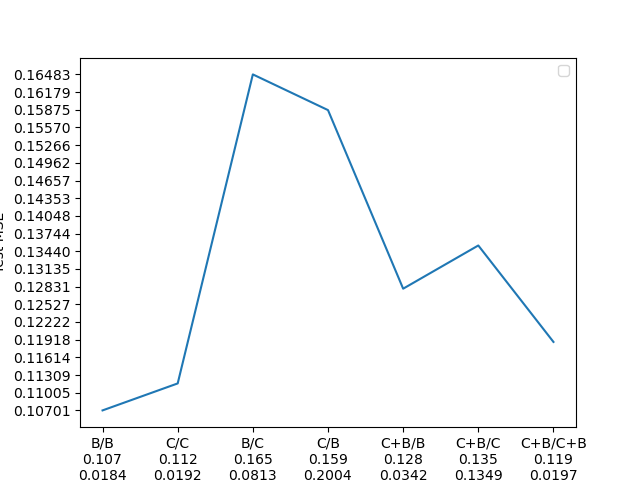
\includegraphics[width=0.3\textwidth]{images/4-0.05.png}
\end{center}
\caption{variational network second order optimization l = 4}
\label{fig:variational}
\end{figure}

\paragraph{Hybrid method}
To help regularize the model we make it resemble the Weidmann model more (ie. we remove the last relu activation and use the exp function). We also use a Weidmann model whose parameters are optimized on the training data and use the distance to it's output with half the weight decay. While it seemed to make sense to use gradient descent here also to get as good an estimate as possible using a simple grid search to get the Weidmann model parameters seems to also produce a good model for the purposes of regularizing the training of our network. It also seems that when we remove the momentum from our model a much smaller network size presents itself.

\begin{figure}
\begin{center}
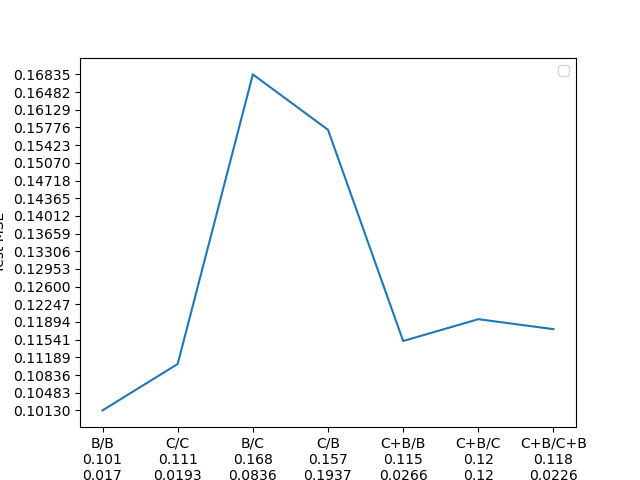
\includegraphics[width=0.3\textwidth]{images/5-5-0.05.png}
\end{center}
\caption{small network (5,5), second order optimization regularization, minumal momentum and regularizing using the knowledge based model}
\label{fig:hybrid}
\end{figure}

\begin{figure}
\begin{center}
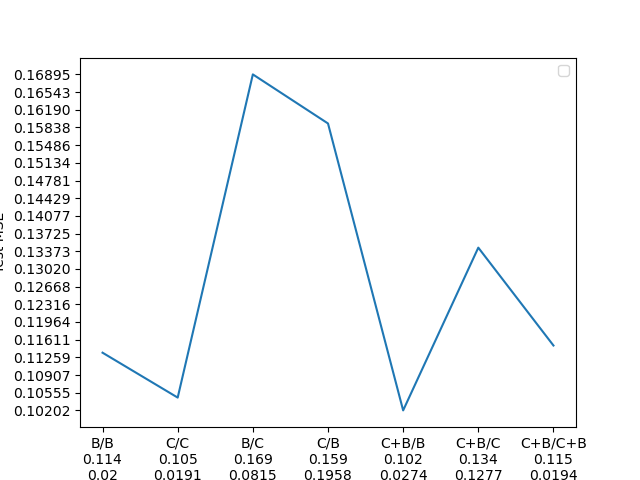
\includegraphics[width=0.3\textwidth]{images/5-5.png}
\end{center}
\caption{small network (5,5), second order optimization regularization, minimal momentum and regularizing using the knowledge based model evaluated on the data prepared with the procedure from the paper}
\label{fig:hybridoriginal}
\end{figure}


\begin{figure}
\begin{center}
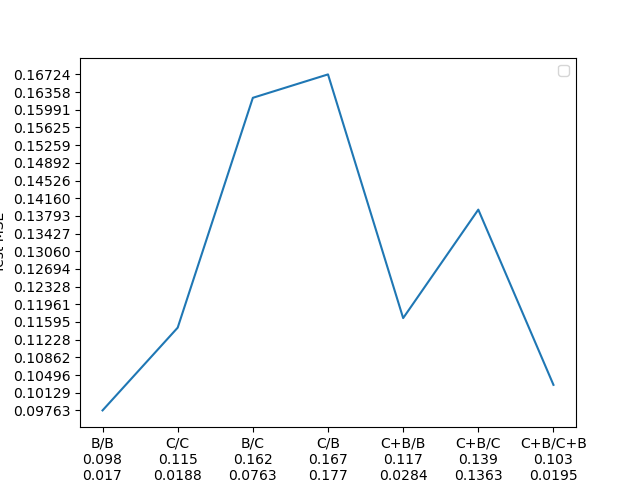
\includegraphics[width=0.3\textwidth]{images/5-5-0.09.png}
\end{center}
\caption{small network (5,5), second order optimization regularization, minimal momentum evaluated on the data prepared with the procedure from the paper}
\label{fig:secondorderoriginal}
\end{figure}

We can see in Figure \ref{fig:hybrid} that the hybrid model as we implemented it did not significantly improve performance. When we look at the experiments done on the original data we see that it outperforms the models in Figure \ref{fig:hybridoriginal} but when we take away the knowledge based regularization (Figure \ref{fig:secondorderoriginal}) it seems that it was not the determining factor.

\paragraph{Conclusion} It seems with the selected data processing methods the choice of architecture did not matter much. However the second order optimization seems to have improved the loss by a small margin. In spite of having the more or less the same relative results between models, our losses for the recreation of the conditions in the paper are significantly higher than the ones in the paper. It is difficult to know why exactly, as the paper did not publish any of their training details like number of epochs, learning rate or weight decay.

\end{task}